\chapter{The Cemetery of the Château d’If}

On the bed, at full length, and faintly illuminated by the pale light
that came from the window, lay a sack of canvas, and under its rude
folds was stretched a long and stiffened form; it was Faria’s last
winding-sheet,—a winding-sheet which, as the turnkey said, cost so
little. Everything was in readiness. A barrier had been placed between
Dantès and his old friend. No longer could Edmond look into those
wide-open eyes which had seemed to be penetrating the mysteries of
death; no longer could he clasp the hand which had done so much to make
his existence blessed. Faria, the beneficent and cheerful companion,
with whom he was accustomed to live so intimately, no longer breathed.
He seated himself on the edge of that terrible bed, and fell into
melancholy and gloomy reverie.

Alone! he was alone again! again condemned to silence—again face to
face with nothingness! Alone!—never again to see the face, never again
to hear the voice of the only human being who united him to earth! Was
not Faria’s fate the better, after all—to solve the problem of life at
its source, even at the risk of horrible suffering?

The idea of suicide, which his friend had driven away and kept away by
his cheerful presence, now hovered like a phantom over the abbé’s dead
body.

“If I could die,” he said, “I should go where he goes, and should
assuredly find him again. But how to die? It is very easy,” he went on
with a smile; “I will remain here, rush on the first person that opens
the door, strangle him, and then they will guillotine me.”

But excessive grief is like a storm at sea, where the frail bark is
tossed from the depths to the top of the wave. Dantès recoiled from the
idea of so infamous a death, and passed suddenly from despair to an
ardent desire for life and liberty.

“Die? oh, no,” he exclaimed—“not die now, after having lived and
suffered so long and so much! Die? yes, had I died years ago; but now
to die would be, indeed, to give way to the sarcasm of destiny. No, I
want to live; I shall struggle to the very last; I will yet win back
the happiness of which I have been deprived. Before I die I must not
forget that I have my executioners to punish, and perhaps, too, who
knows, some friends to reward. Yet they will forget me here, and I
shall die in my dungeon like Faria.”

As he said this, he became silent and gazed straight before him like
one overwhelmed with a strange and amazing thought. Suddenly he arose,
lifted his hand to his brow as if his brain were giddy, paced twice or
thrice round the dungeon, and then paused abruptly by the bed.

“Just God!” he muttered, “whence comes this thought? Is it from thee?
Since none but the dead pass freely from this dungeon, let me take the
place of the dead!”

Without giving himself time to reconsider his decision, and, indeed,
that he might not allow his thoughts to be distracted from his
desperate resolution, he bent over the appalling shroud, opened it with
the knife which Faria had made, drew the corpse from the sack, and bore
it along the tunnel to his own chamber, laid it on his couch, tied
around its head the rag he wore at night around his own, covered it
with his counterpane, once again kissed the ice-cold brow, and tried
vainly to close the resisting eyes, which glared horribly, turned the
head towards the wall, so that the jailer might, when he brought the
evening meal, believe that he was asleep, as was his frequent custom;
entered the tunnel again, drew the bed against the wall, returned to
the other cell, took from the hiding-place the needle and thread, flung
off his rags, that they might feel only naked flesh beneath the coarse
canvas, and getting inside the sack, placed himself in the posture in
which the dead body had been laid, and sewed up the mouth of the sack
from the inside.

He would have been discovered by the beating of his heart, if by any
mischance the jailers had entered at that moment. Dantès might have
waited until the evening visit was over, but he was afraid that the
governor would change his mind, and order the dead body to be removed
earlier. In that case his last hope would have been destroyed.

Now his plans were fully made, and this is what he intended to do. If
while he was being carried out the grave-diggers should discover that
they were bearing a live instead of a dead body, Dantès did not intend
to give them time to recognize him, but with a sudden cut of the knife,
he meant to open the sack from top to bottom, and, profiting by their
alarm, escape; if they tried to catch him, he would use his knife to
better purpose.

\begin{figure}[ht]
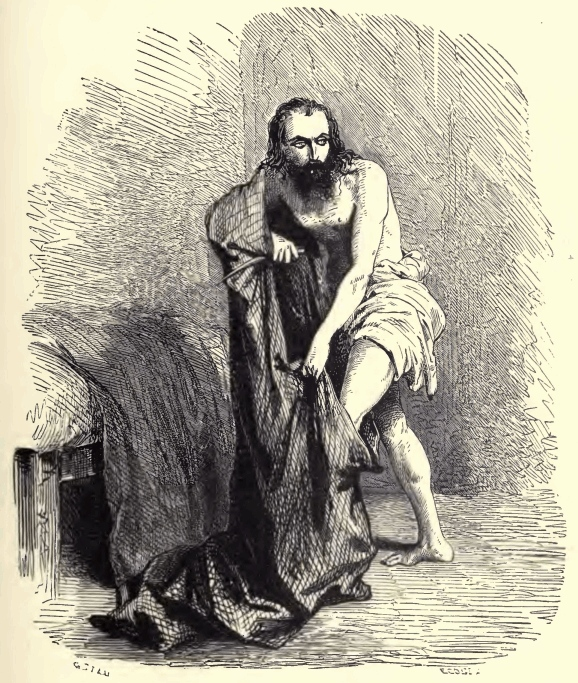
\includegraphics[width=\textwidth]{0263m.jpg}
\end{figure}

If they took him to the cemetery and laid him in a grave, he would
allow himself to be covered with earth, and then, as it was night, the
grave-diggers could scarcely have turned their backs before he would
have worked his way through the yielding soil and escaped. He hoped
that the weight of earth would not be so great that he could not
overcome it. If he was detected in this and the earth proved too heavy,
he would be stifled, and then—so much the better, all would be over.

Dantès had not eaten since the preceding evening, but he had not
thought of hunger, nor did he think of it now. His situation was too
precarious to allow him even time to reflect on any thought but one.

The first risk that Dantès ran was, that the jailer, when he brought
him his supper at seven o’clock, might perceive the change that had
been made; fortunately, twenty times at least, from misanthropy or
fatigue, Dantès had received his jailer in bed, and then the man placed
his bread and soup on the table, and went away without saying a word.
This time the jailer might not be as silent as usual, but speak to
Dantès, and seeing that he received no reply, go to the bed, and thus
discover all.

When seven o’clock came, Dantès’ agony really began. His hand placed
upon his heart was unable to redress its throbbings, while, with the
other he wiped the perspiration from his temples. From time to time
chills ran through his whole body, and clutched his heart in a grasp of
ice. Then he thought he was going to die. Yet the hours passed on
without any unusual disturbance, and Dantès knew that he had escaped
the first peril. It was a good augury.

At length, about the hour the governor had appointed, footsteps were
heard on the stairs. Edmond felt that the moment had arrived, summoned
up all his courage, held his breath, and would have been happy if at
the same time he could have repressed the throbbing of his veins. The
footsteps—they were double—paused at the door—and Dantès guessed that
the two grave-diggers had come to seek him—this idea was soon converted
into certainty, when he heard the noise they made in putting down the
hand-bier.

The door opened, and a dim light reached Dantès’ eyes through the
coarse sack that covered him; he saw two shadows approach his bed, a
third remaining at the door with a torch in its hand. The two men,
approaching the ends of the bed, took the sack by its extremities.

“He’s heavy, though, for an old and thin man,” said one, as he raised
the head.

“They say every year adds half a pound to the weight of the bones,”
said another, lifting the feet.

“Have you tied the knot?” inquired the first speaker.

“What would be the use of carrying so much more weight?” was the reply,
“I can do that when we get there.”

“Yes, you’re right,” replied the companion.

“What’s the knot for?” thought Dantès.

They deposited the supposed corpse on the bier. Edmond stiffened
himself in order to play the part of a dead man, and then the party,
lighted by the man with the torch, who went first, ascended the stairs.
Suddenly he felt the fresh and sharp night air, and Dantès knew that
the mistral was blowing. It was a sensation in which pleasure and pain
were strangely mingled.

The bearers went on for twenty paces, then stopped, putting the bier
down on the ground. One of them went away, and Dantès heard his shoes
striking on the pavement.

“Where am I?” he asked himself.

“Really, he is by no means a light load!” said the other bearer,
sitting on the edge of the hand-barrow.

Dantès’ first impulse was to escape, but fortunately he did not attempt
it.

“Give us a light,” said the other bearer, “or I shall never find what I
am looking for.”

The man with the torch complied, although not asked in the most polite
terms.

“What can he be looking for?” thought Edmond. “The spade, perhaps.”

An exclamation of satisfaction indicated that the grave-digger had
found the object of his search. “Here it is at last,” he said, “not
without some trouble, though.”

“Yes,” was the answer, “but it has lost nothing by waiting.”

As he said this, the man came towards Edmond, who heard a heavy
metallic substance laid down beside him, and at the same moment a cord
was fastened round his feet with sudden and painful violence.

“Well, have you tied the knot?” inquired the grave-digger, who was
looking on.

“Yes, and pretty tight too, I can tell you,” was the answer.

“Move on, then.” And the bier was lifted once more, and they proceeded.

They advanced fifty paces farther, and then stopped to open a door,
then went forward again. The noise of the waves dashing against the
rocks on which the château is built, reached Dantès’ ear distinctly as
they went forward.

“Bad weather!” observed one of the bearers; “not a pleasant night for a
dip in the sea.”

“Why, yes, the abbé runs a chance of being wet,” said the other; and
then there was a burst of brutal laughter.

Dantès did not comprehend the jest, but his hair stood erect on his
head.

“Well, here we are at last,” said one of them.

“A little farther—a little farther,” said the other. “You know very
well that the last was stopped on his way, dashed on the rocks, and the
governor told us next day that we were careless fellows.”

They ascended five or six more steps, and then Dantès felt that they
took him, one by the head and the other by the heels, and swung him to
and fro.

“One!” said the grave-diggers, “two! three!”

And at the same instant Dantès felt himself flung into the air like a
wounded bird, falling, falling, with a rapidity that made his blood
curdle. Although drawn downwards by the heavy weight which hastened his
rapid descent, it seemed to him as if the fall lasted for a century. At
last, with a horrible splash, he darted like an arrow into the ice-cold
water, and as he did so he uttered a shrill cry, stifled in a moment by
his immersion beneath the waves.

Dantès had been flung into the sea, and was dragged into its depths by
a thirty-six-pound shot tied to his feet.

The sea is the cemetery of the Château d’If.

\begin{figure}[h]
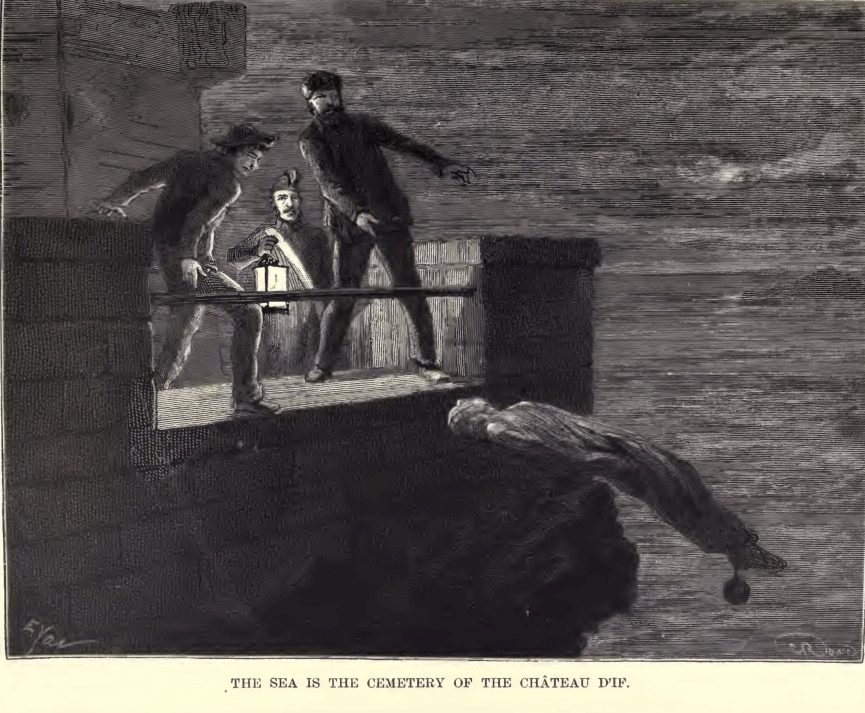
\includegraphics[width=\textwidth]{0267m.jpg}
\end{figure}
